\chapter{Ajuster un modèle de régression linéaire simple (RLS)}
\label{sec:AjusterRLS}

\section{Le modèle de régression linéaire simple}
\label{sec:ModèleRLS}

Le modèle de régression linéaire simple est un modèle dans lequel on cherche à expliquer une variable endogène $Y$ en fonction d'une seule variable exogène $x$. Il s'exprime comme suit:
\begin{eqnarray}
 Y_i = \beta_0 + \beta_1 x_i + \varepsilon_i, \ \ \ \ \ \ \ 1\leq i \leq n.
 \label{eq:reg_lin_simple}
\end{eqnarray}
où $Y_1,\ldots,Y_n$ sont $n$ observations de la variable endogène (variable réponse);\\
$x_1,\ldots,x_n$ sont $n$ observations de la variable exogène (variable explicative);\\
$\beta_0$ est le paramètre associé à l'ordonnée à l'origine de la droite;\\
$\beta_1$ est le paramètre associé à la pente de la droite;\\
$\varepsilon_1,\ldots,\varepsilon_n$ sont des termes d'erreurs;\\
et $n$ est le nombre d'observations.\\

\begin{remarque}
Il est important de comprendre quelles grandeurs sont supposées constantes ou aléatoires dans le modèle \eqref{eq:reg_lin_simple}, à savoir
 \begin{itemize}
 \item[$\bullet$]
 $Y_1,\ldots, Y_n$ sont les réalisations connues d'une variable aléatoire;
 \item[$\bullet$]
 $x_1,\ldots,x_n$ sont des valeurs connues et considérées constantes;
 \item[$\bullet$]
 $\beta_0$ et $\beta_1$, les paramètres du modèle, sont constants, mais inconnus, et il faudra par conséquent les estimer;
 \item[$\bullet$] $\varepsilon_1,\ldots,\varepsilon_n$ sont les réalisations inconnues d'une variable aléatoire.
  \end{itemize}
\end{remarque}

\subsection{Postulats du modèle de RLS}
\label{sec:Postulats}

Pour développer la théorie de la régression linéaire, il sera nécessaire de formuler certains postulats supplémentaires au modèle défini en \ref{eq:reg_lin_simple}.

Les trois principaux postulats, ou conditions d'application, sont les suivants:
\begin{enumerate}
  \item[$\mathcal{P}_1$.] La linéarité de la relation entre la variable endogène et la variable exogène.
 \item[$\mathcal{P}_2$.] L'homoscédasticité (variance constante) des observations de la variable endogène.
 \item[$\mathcal{P}_3$.] L'indépendance des observations de la variable endogène.
\end{enumerate}

Le premier postulat est nécessaire pour l'interprétation des paramètres du modèle, et indique simplement que le modèle linéaire est approprié pour modéliser la relation entre les variables d'intérêt. Les deux autres postulats %ne sont pas aussi essentiels à l'utilisation du modèle de régression linéaire simple, mais on verra à la \autoref{sec:InférenceParamètres} qu'ils 
permettent d'estimer la variance des estimateurs de $\beta_0$ et $\beta_1$. Obtenir une telle mesure de précision des estimateurs ponctuels est très important en pratique.

Ces trois postulats peuvent être énoncés mathématiquement en termes d'hypothèses sur les termes d'erreur $\varepsilon_i$ du modèle \eqref{eq:reg_lin_simple}:
\begin{align*}
\mathcal{P}_1. & \; \; \esp[\varepsilon_i]=0 \mbox{ pour } 1\leq i \leq n\\
\mathcal{P}_2. & \; \; \var[\varepsilon_i]=\sigma^2 \mbox{ pour } 1\leq i \leq n\\
\mathcal{P}_3. & \; \; \cov(\varepsilon_i,\varepsilon_j)=0 \mbox{ pour } i \neq j
\end{align*}

À ces trois postulats, on doit parfois ajouter l'hypothèse de normalité des résidus :
$$ \mathcal{P}_4. \;\varepsilon_1, \cdots , \varepsilon_n \sim \N(0,\sigma^2)$$
Il s'agit d'un postulat plus fort généralement utilisé parce qu'il permet de construire des intervalles de confiance et de faire des tests d'hypothèses aisément\footnote{Il est également possible d'obtenir des intervalles de confiance et des tests d'hypothèses sans poser le postulat de normalité des erreurs, en utilisant par exemple la méthode du bootstrap.}. On verra également que ce postulat est nécessaire à la mise en {\oe}uvre de la méthode du maximum de vraisemblance pour l'estimation des paramètres.

Il est évidemment possible que ces 4 postulats ne soient pas vérifiés en pratique. Nous verrons à la \autoref{sec:transfoRLS} comment tester si chacun des postulats est vérifié et comment modifier le modèle au besoin. Le \autoref{sec:TechniquesAvancees} décrit en outre certains autres modèles de régression qui peuvent être utilisés si une ou plusieurs des conditions d'application de la RLS ne sont pas vérifiées.


\subsection{Interprétation de $\beta_0$ et $\beta_1$}
\label{sec:Interprétation}


La \autoref{fig:rls} illustre le modèle de régression linéaire simple. La ligne droite représente la valeur moyenne de $Y$ en fonction de la valeur de $x$. Les valeurs observées de $Y$ sont distribuées de façon aléatoire autour de cette droite. Les termes d'erreur sont les différences entre les valeurs observées de $Y$ et la droite. Comme la variance de ces termes est constante en $x$, la distance moyenne des points à la droite est la même pour toute valeur de $x$. Finalement, l'absence de corrélation entre les termes d'erreur
signifie que la valeur d'un terme d'erreur n'est pas influencée par la valeur des autres termes d'erreur.

\begin{figure}[h!]
\centerline{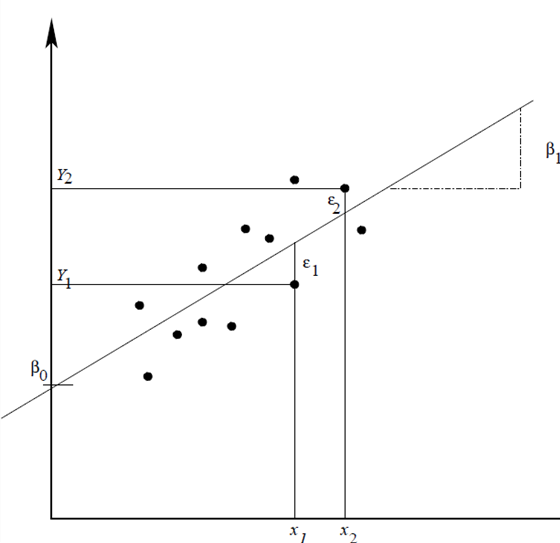
\includegraphics[scale=1]{Chap2-AjusterRLS/Figures/schema_reg_lin}}
\caption[Illustration du modèle de régression linéaire simple]{Illustration du mod\`ele de r\'egression lin\'eaire simple. La droite repr\'esente l'esp\'erance de la
variable endog\`ene, $Y$, en fonction de la valeur de la variable
exog\`ene, $x$. Le param\`etre $\beta_0$ constitue l'ordonn\'ee
\`a l'origine de la droite et le param\`etre $\beta_1$ est égal à la pente de
la droite.}
\label{fig:rls}
\end{figure}


On interprète donc $\beta_0$ comme la valeur moyenne de $Y$ lorsque $x$ vaut zéro et $\beta_1$ comme l'accroissement moyen de $Y$ lorsque $x$ augmente d'une unité. Si $\beta_0 = 0$, l'espérance de $Y$ est nulle lorsque $x$ vaut zéro, et le modèle ne comporte pas d'ordonnée à l'origine. Si $\beta_1 = 0$, l'espérance de $Y$ ne dépend pas de $x$, du moins pas de façon linéaire.

\newpage
\textbf{Modèle centré}

Il arrive que la valeur moyenne de $Y$ lorsque $x$ vaut zéro soit difficile ou inutile à interpréter. On pourra alors utiliser une version centrée du modèle:
\begin{eqnarray*}
 Y_i &=& \beta_0 + \beta_1 x_i + \varepsilon_i \\
 &=& \beta_0^* + \beta_1 (x_i - \overline{x}) + \varepsilon_i \text{ (version centrée)}
\end{eqnarray*}

Dans la version centrée du modèle, l'interprétation de $\beta_1$ est inchangée, mais $\beta_0^*$ s'interprète comme étant la valeur moyenne de $Y$ lorsque $x$ vaut $\overline{x}$. On remarque que $\beta_0^* = \beta_0 + \beta_1 \overline{x}$.


\section{Estimation des paramètres}
\label{sec:estimation}

Dans la régression linéaire simple, on doit estimer trois paramètres: $\beta_0$ et $\beta_1$, qui décrivent la droite de régression, ainsi que $\sigma^2$, la variance des termes d'erreur. Deux approches sont généralement admises pour estimer les paramètres d'un modèle de régression: la méthode des moindres carrés et celle du maximum de vraisemblance. On expliquera comment estimer les paramètres de régression à l'aide de ces deux approches, et on démontrera qu'elles sont équivalentes sous le postulat de normalité $\mathcal{P}_4$.

\subsection{Méthode des moindres carrés}

Tel que mentionné au \autoref{sec:intro}, on attribue généralement la méthode des moindres carrés au mathématicien français Adrien-Marie Legendre (1752-1833). Plusieurs autres mathématiciens de l'époque ont aussi publié des travaux sur le sujet, notamment Carl Friedrich Gauss (1777-1855) et Robert Adrain (1775-1843).

Soit $\hat{Y}_i$ la prévision du modèle pour l'observation $i$, c'est-à-dire la position de $Y_i$ s'il était exactement sur la droite de régression. On appelle résidu la différence entre $Y_i$, la valeur observée de la variable réponse, et cette prévision $\hat{Y}_i$. On le dénote $\hat{\varepsilon}_i$, puisque c'est une estimation du terme d'erreur $\varepsilon_i$.

Avec la méthode des moindres carrés, on cherche à choisir $\hat\beta_0$ et $\hat\beta_1$ de façon à minimiser la somme des carrés des erreurs. On veut donc minimiser la fonction suivante:
\begin{eqnarray}
g(\beta_0,\beta_1) =  \sum_{i=1}^n \varepsilon_i^2  =  \sum_{i=1}^n \left\{Y_i- (\beta_0+\beta_1 x_i)\right\}^2
    \label{eq:MoindresCarres}
\end{eqnarray}

Puisque la fonction \`a minimiser possède de bonnes propri\'et\'es
(entre autres lisse et convexe), elle peut être minimisée en la dérivant par rapport \`a ${\beta}_0$ et ${\beta}_1$, puis en posant ces d\'eriv\'ees \'egales \`a z\'ero. On doit donc résoudre le système d'équations \`a deux inconnues suivant:
\begin{eqnarray}
\left\{ \begin{array}{ccc}
\frac{\partial}{\partial{\beta}_0}
\sum_{i=1}^n(Y_i-{\beta}_0-{\beta}_1 x_i)^2
&=&\label{eq1} 0 \\
\frac{\partial}{\partial{\beta}_1}
\sum_{i=1}^n(Y_i-{\beta}_0-{\beta}_1 x_i)^2
&=&\label{eq2} 0
\end{array}
\right.
\end{eqnarray}

\textbf{Estimation de $\beta_0$}

On dérive d'abord par rapport à $\beta_0$:
\begin{eqnarray*}
 \frac{\partial}{\partial \beta_0} \left\{\sum_{i=1}^n (Y_i - \beta_0 - \beta_1 x_i)^2\right\} &=& \sum_{i=1}^n 2(Y_i - \beta_0 - \beta_1 x_i)(-1)\\
 &=& -2( n \overline{Y} - n \beta_0 - n \beta_1 \overline{x})
\end{eqnarray*}
On pose ensuite cette dérivée égale à zéro, d'où l'apparition des chapeaux, car il s'agit du point critique de la fonction $g(\beta_0,\,\beta_1)$:
\begin{eqnarray}
-2(n \overline{Y} - n \hat\beta_0 - n \hat\beta_1 \overline{x}) & = & 0 \nonumber\\
 \overline{Y} - \hat\beta_0 - \hat\beta_1 \overline{x} & = & 0 \nonumber\\
 \hat\beta_0 & = &  \overline{Y} - \hat\beta_1 \overline{x}
\label{eq:beta0}
\end{eqnarray}


\begin{remarque}
 Il est à noter que l'équation \eqref{eq:beta0} signifie que la droite de régression passe nécessairement par le point de coordonnées $(\overline{x},\overline{Y})$:

\begin{eqnarray}
\overline{Y} = \hat\beta_0+ \hat\beta_1 \overline{x}
 \label{eq:dbeta0egal0}
\end{eqnarray}
\end{remarque}

\textbf{Estimation de $\beta_1$}

On dérive maintenant par rapport à $\beta_1$:
\begin{eqnarray*}
 \frac{\partial}{\partial \beta_1} \left\{\sum_{i=1}^n (Y_i - \beta_0 - \beta_1 x_i)^2\right\} &=& \sum_{i=1}^n 2(Y_i - \beta_0 - \beta_1 x_i)(-x_i)\\
 &=& -2 \left(\sum_{i=1}^n x_i Y_i - \sum_{i=1}^n  \beta_0 x_i - \sum_{i=1}^n  \beta_1 x_i^2 \right).
\end{eqnarray*}

\newpage
En posant cette dérivée égale à zéro et en utilisant  \eqref{eq:beta0}, on a
\begin{eqnarray*}
-2 \left( \sum_{i=1}^n x_i Y_i - \sum_{i=1}^n  \hat\beta_0 x_i - \sum_{i=1}^n  \hat\beta_1 x_i^2\right) & = & 0 \\
\sum_{i=1}^n x_i Y_i &= & \hat\beta_0 \sum_{i=1}^n x_i + \hat\beta_1 \sum_{i=1}^nx_i^2 \\
\sum_{i=1}^n x_i Y_i & = & (\overline{Y}-\hat\beta_1 \overline{x}) \sum_{i=1}^n x_i + \hat\beta_1 \sum_{i=1}^nx_i^2 \\
\sum_{i=1}^n x_i Y_i & = & \overline{Y} \sum_{i=1}^n x_i + \hat\beta_1 \left(\sum_{i=1}^n x_i^2 - \overline{x}\sum_{i=1}^n x_i \right)
\end{eqnarray*}

On obtient donc l'estimateur suivant:
\begin{equation}
\hat{\beta}_1 = \frac{\sum_{i=1}^n x_i Y_i -\overline{Y} \sum_{i=1}^n x_i}{\sum_{i=1}^n x_i^2 - \overline{x}\sum_{i=1}^n x_i}.
\end{equation}


Il est possible ensuite de réécrire $\hat\beta_1$ sous les formes équivalentes suivantes:
\begin{equation*}
 \hat{\beta}_1 =  \frac{\sum_{i=1}^n x_i Y_i - n\overline{x}\overline{Y}}{\sum_{i=1}^n x_i^2 - n\overline{x}^2}
 = \frac{\sum_{i=1}^n (x_i-\overline{x})(Y_i-\overline{Y})}{\sum_{i=1}^n (x_i-\overline{x})^2}
 = \frac{\sum_{i=1}^n (x_i-\overline{x})Y_i}{\sum_{i=1}^n (x_i-\overline{x})^2}
 \label{eq:beta1}
\end{equation*}

Chacune pourra être utile pour calculer $\hat{\beta_1}$ selon le type d'information que nous avons sur les données. On simplifie parfois davantage la notation en écrivant
\begin{equation}
 \hat{\beta}_1  = \frac{S_{xy}}{S_{xx}}
\end{equation}
o\`u
\begin{eqnarray}
S_{xy}=\sum_{i=1}^n (x_i-\overline x)\,Y_i=\sum_{i=1}^nx_iY_i-\frac{1}{n}\left(\sum_{i=1}^n x_i\right)\left(\sum_{i=1}^n Y_i\right)
\label{eq:Sxy}
\end{eqnarray}
\begin{eqnarray}
S_{xx}=\sum_{i=1}^n(x_i-\overline x)^2=\sum_{i=1}^nx_i^2-\frac{1}{n}\left(\sum_{i=1}^n x_i\right)^2
\label{eq:Sxx}
\end{eqnarray}
Il est à noter que $S_{xy}$ et $S_{xx}$ sont appelés respectivement la somme des produits croisés corrigée de $x$ et $Y$ et la somme des carrés corrigée de $x$.


En somme, les estimateurs des moindres carrés pour la RLS sont
\begin{eqnarray}
\hat \beta_1 = \frac{S_{xy}}{S_{xx}} & \hspace{2cm} & \hat\beta_0=\overline{Y} - \hat\beta_1 \overline{x}
\end{eqnarray}


%On ne poursuit pas les développements mathématiques nécessaires pour obtenir ces estimateurs ici. On montrera à la section suivante que la méthode des moindres carrés est équivalente à la méthode du maximum de vraisemblance sous le postulat de normalité, et on montrera alors comment obtenir les estimateurs.

\subsection{Méthode du maximum de vraisemblance}

La méthode du maximum de vraisemblance nécessite de spécifier la distribution exacte des observations $Y_1,\dots, Y_n$. Celle-ci est connue sous l'hypothèse des quatre postulats
\begin{align*}
\mathcal{P}_1. & \; \; \esp[\varepsilon_i]=0 \mbox{ pour } 1\leq i \leq n
&
\mathcal{P}_3. & \; \; \cov(\varepsilon_i,\varepsilon_j)=0 \mbox{ pour } i \neq j \\
\mathcal{P}_2. & \; \; \var[\varepsilon_i]=\sigma^2 \mbox{ pour } 1\leq i \leq n
&
\mathcal{P}_4. & \;\varepsilon_1, \cdots , \varepsilon_n \sim \N(0,\sigma^2)
\end{align*}
En effet, on peut alors écrire le modèle sous la forme
\begin{align*}
Y_i &= \beta_0 + \beta_1 x_i + \varepsilon_i, \ \ \  \varepsilon_i \iid N(0,\sigma^2) \ \ \ \ 1\leq i \leq n
 \end{align*}
ou, de façon équivalente
\begin{equation}
Y_i \sim N(\beta_0 + \beta_1 x_i, \sigma^2)
\end{equation}

La vraisemblance s'exprime donc
\begin{eqnarray*}
 L (\beta_0, \beta_1, \sigma^2)&=&\prod_{i=1} ^n f(Y_i) \\
 &=& \prod_{i=1} ^n \frac{1}{\sqrt{2\pi}\sigma} \exp\left\{-\frac{1}{2} \left(\frac{Y_i-\beta_0 - \beta_1 x_i}{\sigma}\right)^2\right\}.
\end{eqnarray*}

 Il reste ensuite à maximiser la fonction $L (\beta_0, \beta_1)$ ou, plus simplement, son logarithme
 \begin{eqnarray}
 \nonumber l (\beta_0, \beta_1, \sigma^2)&=&\sum_{i=1}^n \left\{-\frac{1}{2}\log(2\pi\sigma^2)-\frac{1}{2\sigma^2}(Y_i - \beta_0 - \beta_1 x_i)^2\right\}\\ \label{eq:MaxVraisemblance}
 &=& -\frac{n}{2} \log (2\pi\sigma^2)-\frac{1}{2 \sigma^2}\sum_{i=1}^n (Y_i - \beta_0 - \beta_1 x_i)^2
\end{eqnarray}

On trouve $\hat\beta_0$, $\hat\beta_1$ et $\hat\sigma^2$ qui minimisent $l (\beta_0, \beta_1,\sigma^2)$ en dérivant respectivement par rapport à $\beta_0,\beta_1$ et $\sigma^2$ puis en posant les dérivées égales à zéro.

%\begin{remarque}
Dans l'équation \eqref{eq:MaxVraisemblance}, on remarque que le premier terme ne contient ni $\beta_0$, ni $\beta_1$. Maximiser la log-vraisemblance par rapport à $\beta_0$ et $\beta_1$ revient donc à maximiser le second terme. Ce dernier étant négatif, cela équivaut à minimiser $\sum_{i=1}^n (Y_i - \beta_0 - \beta_1 x_i)^2$, ce qui correspond exactement à la méthode des moindres carrés de Legendre.  Ainsi, les estimateurs de la méthode du maximum de vraisemblance de $\beta_0$ et $\beta_1$ sont les mêmes qu'avec la méthode des moindres carrés.

La méthode du maximum de vraisemblance présente toutefois certains avantages par rapport à la méthode des moindres carrés. Elle permet notamment d'estimer $\sigma^2$ de façon directe. Ceci permet de trouver la distribution des paramètres et des prévisions et de faire des tests d'hypothèse, comme on verra dans les sections suivantes.
%\end{remarque}

\subsubsection{Estimation de $\sigma^2$}
On estime $\sigma^2$ de la même manière que $\beta_0$ et $\beta_1$ en dérivant le logarithme de la vraisemblance par rapport à $\sigma^2$.
 \begin{eqnarray*}
 \frac{\partial}{\partial \sigma^2}\left\{ -\frac{n}{2} \log (2\pi\sigma^2)-\frac{1}{2 \sigma^2}\sum_{i=1}^n (Y_i - \beta_0 - \beta_1 x_i)^2\right\}
 & = & -\frac{n}{2} \frac{1}{2\pi\sigma^2} 2\pi + \frac{1}{\sigma^4} \frac{1}{2}\sum_{i=1}^n(Y_i-\beta_0-\beta_1 x_i)^2 \\
 & = & -\frac{n}{2\sigma^2}+ \frac{1}{2 \sigma^4}\sum_{i=1}^n(Y_i-\beta_0-\beta_1 x_i)^2
\end{eqnarray*}

En posant la dérivée égale à zéro et en remplaçant les paramètres $\beta_0$ et $\beta_1$ par leurs estimateurs, on a :
\begin{equation}
 \hat{\sigma}^2_{MV} = \frac{1}{n}\sum_{i=1}^n(Y_i - \hat{\beta_0} - \hat{\beta_1}x_i)^2 = \frac{1}{n}\sum_{i=1}^n \hat{\varepsilon_i}^2
 \label{sigma2}
\end{equation}

Rappelons que $\hat{\varepsilon_i}$ désigne l'estimation du terme d'erreur, que l'on nomme résidu.

\section{Exemple}
\label{exemple-RLS-interpretation}
Le petit exemple qui va servir de fil conducteur pour les chapitres sur la régression linéaire simple est tiré de \citet[Exemple 13.1, page 367]{Hin_Mon_Gol_Bor:05}. Un ingénieur chimiste a analysé l'effet de la température de fonctionnement d'un procédé sur le rendement du produit. Les valeurs obtenues sont résumées ci-dessous.


\begin{table}[!ht]
\caption{10 mesures du rendement en $\%$ en fonction de la température en $^{\circ}\mathrm{C}$ } \label{tab:donnees_exp}
\label{exp:donnees}
\begin{tabular}{r|rrrrrrrrrr}
Température [$^{\circ}\mathrm{C}$] & 100 & 110 & 120 & 130 & 140 & 150 & 160 & 170 & 180 & 190 \\[6pt] \hline
\\[-6pt]
Rendement [$\%$] & 45 & 51 & 54 & 61 & 66 & 70 & 74 & 78 & 85 & 89
\end{tabular}
\end{table}

\begin{figure}[h!]
\centering
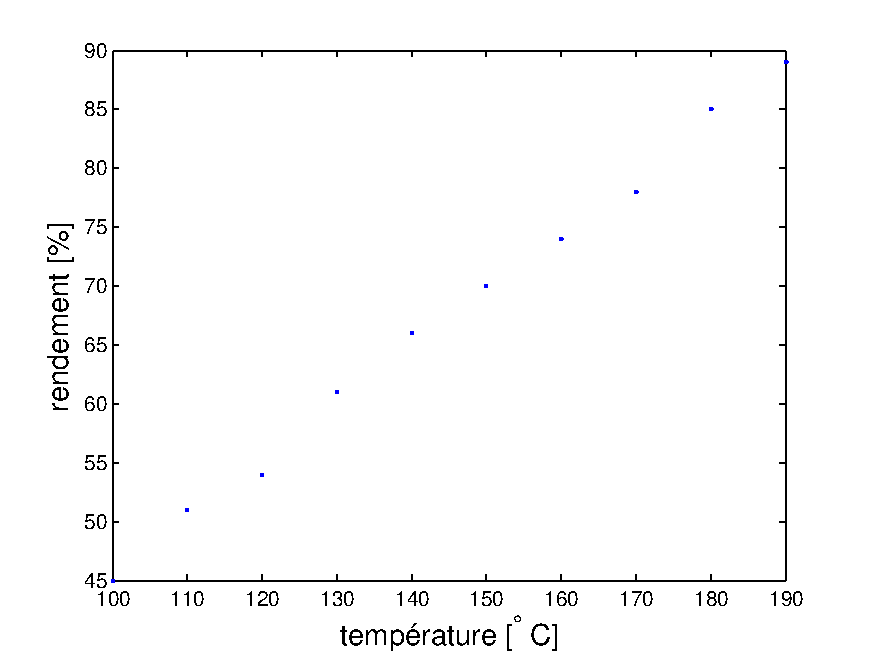
\includegraphics[scale=0.6]{Chap2-AjusterRLS/Figures/scatter_plot_exp.pdf}
\caption{Diagramme de dispersion du rendement en fonction de la température}
\label{fig:scatter_plot_exp}
\end{figure}

On peut constater sur la figure \ref{fig:scatter_plot_exp} qu'il existe une relation forte entre le rendement et la température. On va supposer que cette relation est linéaire et donc modéliser ces données à l'aide de l'équation \eqref{eq:reg_lin_simple}. On calcule d'abord
\begin{align*}
 \sum_{i=1}^{10} x_i &=1450 &\hspace{1cm} & \overline{x}= \frac{1}{10} \sum_{i=1}^{10} x_i=145 & \sum_{i=1}^{10} x_i^2 = 218~500\\
  \sum_{i=1}^{10} y_i&=673 &\hspace{1cm} & \overline{y}= \frac{1}{10} \sum_{i=1}^{10} y_i=67,3 & \sum_{i=1}^{10} Y_ix_i= 101~570
\end{align*}
On obtient alors
\vspace{-0.1 in}
\begin{align*}
S_{xx}&=218~500-(1450)^2/10=8250 \\
S_{xy}&=101~570-1450\times 673/10=3985
\end{align*}
Et donc
\vspace{-0.1 in}
\begin{align*}
\hat{\beta_1} &= 3985/8250=0,483 \\
\hat{\beta_0} &= 67,3-0,483\times145=-2,739
\end{align*}
Le modèle de régression linéaire simple ajusté devient alors $\hat Y_i=-2,739+0,483x_i$. Ainsi, une augmentation de un degré Celsius de la température du procédé est associée à une augmentation moyenne de $0,483$ point de pourcentage du rendement du produit. Le modèle indique aussi qu'à une température nulle, le rendement attendu est de $-2,739\%$.

La figure~\ref{fig:reg_lin_exp} montre l'ajustement obtenu sous forme d'une droite. Dans ce cas-ci la relation linéaire semble très appropriée pour modéliser la relation entre les variables, mais ce ne sera pas toujours le cas.

\begin{figure}[h!]
\centering
\includegraphics[scale=0.6]{Chap2-AjusterRLS/Figures/reg_lin_exp}
\caption{Diagramme de dispersion du rendement en fonction de la température avec la droite de régression estimée superposée}
\label{fig:reg_lin_exp}
\end{figure}

On peut également estimer $\sigma^2$ à partir des données. Il faut d'abord calculer la valeur prédite et le résidu pour chacune des observations, comme au Tableau \ref{tab:cal_sigma2_exp}. L'équation~\eqref{sigma2} livre alors
$$\hat{\sigma}^2_{MV}=\frac{1}{10} \{(-0,561)^2+\cdots+(-0,0301)^2\}=\frac{7,224}{10}=0,7224.$$

\begin{table}[h!]
\caption{Tableau résumant $x_i$, $Y_i$, $\hat Y_i$ et $\hat\varepsilon_i$, $i=1,\dots,10$ pour le calcul de $\hat\sigma^2_{MV}$ dans l'exemple de la section \ref{exemple-RLS-interpretation}}
\label{tab:cal_sigma2_exp}
\begin{center}
\begin{tabular}{c|cccc}
\centering
$i$ & $x_i$& $Y_i$ & $\hat Y_i$ & $\hat\varepsilon_i$ \\ \hline
1 & 100 & 45 & 45,561 &  -0,561 \\
2 & 110  & 51  & 50,391 & 0,609 \\
3 &  120 & 54  & 55,221 & -1,221 \\
4 & 130  & 61 & 60,051 & 0,949\\
5 & 140 & 66  & 64,881  &  1,119 \\
6 & 150  & 70 & 69,711  & 0,289\\
7 &160  & 74 & 74,541 & -0,541\\
8 & 170  & 78 & 79,371 & -1,371\\
9 & 180 & 85 & 84,201 & 0,799\\
10 & 190  & 89 & 89,031 & -0,031
\end{tabular}
\end{center}
\end{table}

